\documentclass[conference]{IEEEtran}
\IEEEoverridecommandlockouts
\usepackage{cite}
\usepackage{amsmath,amssymb}
\usepackage{graphicx}
\usepackage{booktabs}
\usepackage{array}
\usepackage{url}
\usepackage[T1]{fontenc}
\graphicspath{{figures/}}
% generous float parameters (figure-heavy systems paper)
\renewcommand{\topfraction}{0.95}
\renewcommand{\bottomfraction}{0.9}
\renewcommand{\textfraction}{0.06}
\renewcommand{\floatpagefraction}{0.85}
\renewcommand{\dbltopfraction}{0.95}
\renewcommand{\dblfloatpagefraction}{0.85}
\setcounter{topnumber}{3}
\setcounter{bottomnumber}{2}
\setcounter{totalnumber}{5}
\setcounter{dbltopnumber}{3}

\begin{document}

\title{Proprioceptive Leg-Entanglement Detection for a Quadruped:\\
A Multi-Task Causal TCN with Per-Leg Attribution\\ and Physics-Grounded Severity}

\author{\IEEEauthorblockN{Saurav Gupta}
\IEEEauthorblockA{\textit{Autonomous Systems Research}\\
Unitree Go2 Deployment Study\\
sauravgupta1375@gmail.com}}

\maketitle

\begin{abstract}
When a quadruped snags a leg on a wire, a table leg, or loose netting, the fault is easy to miss with external cameras or lidar, and the proprioceptive trace it leaves is faint and easily mistaken for ordinary standing or for the rigid post-stand-up ``Lock'' stance. We treat the problem as time-series event detection and train a single multi-task causal temporal convolutional network on a $0.40$~s, $60$-channel window of joint, foot-contact, and inertial signals. The network jointly predicts whether a leg is entangled, which of the four legs is affected, and a per-leg severity in $[0,1]$ that is grounded in a physics index combining a confidence gate, a Mahalanobis deviation from the walking distribution, and resistive thigh effort. Because every output is read from the last timestep of a strictly left-padded (causal) stack, the model validated offline is the one deployed through an ONNX runtime, whose outputs match the research pipeline to within $4\times10^{-7}$, so the architecture introduces no train--deploy gap. On a leakage-safe held-out split grouped by recording, the detector reaches an F1 of $0.809$, a ROC-AUC of $0.956$, and a multi-label exact-match of $0.908$; leave-one-recording-out cross-validation over $15$ folds gives an F1 of $0.807 \pm 0.142$. Inference costs about $1$~ms per window on a single CPU thread. All results are from recorded-log replay; we report offline evaluation only and make no claim of live on-robot detection performance.
\end{abstract}

\begin{IEEEkeywords}
Legged robots, proprioception, entanglement detection, temporal convolutional networks,
multi-task learning, model calibration, ROS\,2.
\end{IEEEkeywords}

\section{Introduction}

Legged robots earn their mobility in exactly the settings that trip them up. A quadruped that can step over a curb or cross rubble is also a quadruped that can hook a foot under a loose cable, snag a calf on a taut wire, or drag a trailing line between its legs. We call this failure \emph{leg entanglement}, and on a walking platform such as the Unitree Go2~\cite{unitree_go2} it is both common and dangerous: the affected leg loses its expected swing, the controller keeps commanding a gait that the physical leg can no longer execute, and the robot lurches, stalls, or falls. Detecting the condition early, and knowing which leg is caught, is a prerequisite for any sensible response.

The obvious sensing route, exteroception, is unusually weak for this problem. Cables and wires are thin, dark, and frequently occluded by the robot's own body or by the very legs they wrap around; the interaction happens below the belly, outside a forward-facing camera's useful field of view, and against cluttered ground. Proprioception is the natural alternative. The joint encoders, joint torques, foot-contact forces, and inertial signals that already drive the walking controller carry a direct mechanical trace of a snag, and proprioceptive signals are routinely used for legged locomotion and state estimation~\cite{hwangbo2019learning,lee2020learning,camurri2017contact}. When a leg is held back, the thigh joint fights a load it cannot move: torque climbs while velocity stays near zero. That is a real signature, and it is the one we build on.

The difficulty is that the signature is subtle and easy to confuse. A high thigh torque at low joint velocity also describes a robot standing still and bearing its own weight, so a naive torque rule fires constantly during ordinary stops. The confusion is sharpest for the rigid ``Lock'' stance the Go2 holds immediately after standing up, where every joint is stiff, torques are large, and motion is nil, yet nothing is wrong. A useful detector therefore cannot simply threshold effort; it must read effort in the temporal context of the gait and separate a genuine snag from a benign, effortful pose.

We frame the task as time-series event detection over the proprioceptive stream and ask three questions at every timestep: \emph{whether} any leg is entangled, \emph{which} of the four legs (front-right, front-left, rear-right, rear-left) it is, and \emph{how severe} the entanglement is. The first is a binary alarm, the second is a per-leg attribution needed to act on the right limb, and the third is a bounded severity index that grades a light brush against a hard snag. Figure~\ref{fig:system} shows how a single causal model answers all three from a short window of on-robot signals, published as a state message for downstream consumers on ROS~2~\cite{macenski2022ros2}. Answering the three jointly, rather than with three unrelated detectors, lets the shared representation carry the temporal context that distinguishes entanglement from standing and from the Lock stance.

This paper makes the following contributions:
\begin{itemize}
  \item A proprioception-only formulation of leg entanglement as a multi-task, per-timestep event-detection problem that jointly answers \emph{whether}, \emph{which}, and \emph{how-severe}, using only signals the walking controller already produces.
  \item A compact causal dilated temporal convolutional network with three heads (detection, per-leg attribution, and a severity auxiliary), together with physics-grounded features that encode the ``high torque, little motion'' snag signature and let the model separate entanglement from standing and from the rigid post-stand-up Lock stance.
  \item A physics-grounded, calibrated per-leg severity index that gates a Mahalanobis deviation from the walking distribution by resistive thigh effort and per-leg confidence, reported as a severity index rather than a measured force.
  \item An evaluation under a leakage-safe, whole-recording split with leave-one-recording-out cross-validation, a rule-based baseline under an identical protocol, feature ablations, and a calibration study, alongside a runtime whose numerical output matches the research pipeline and whose per-window latency sits well under the real-time budget on the deployment CPU.
\end{itemize}
\begin{figure*}[t]
\centering
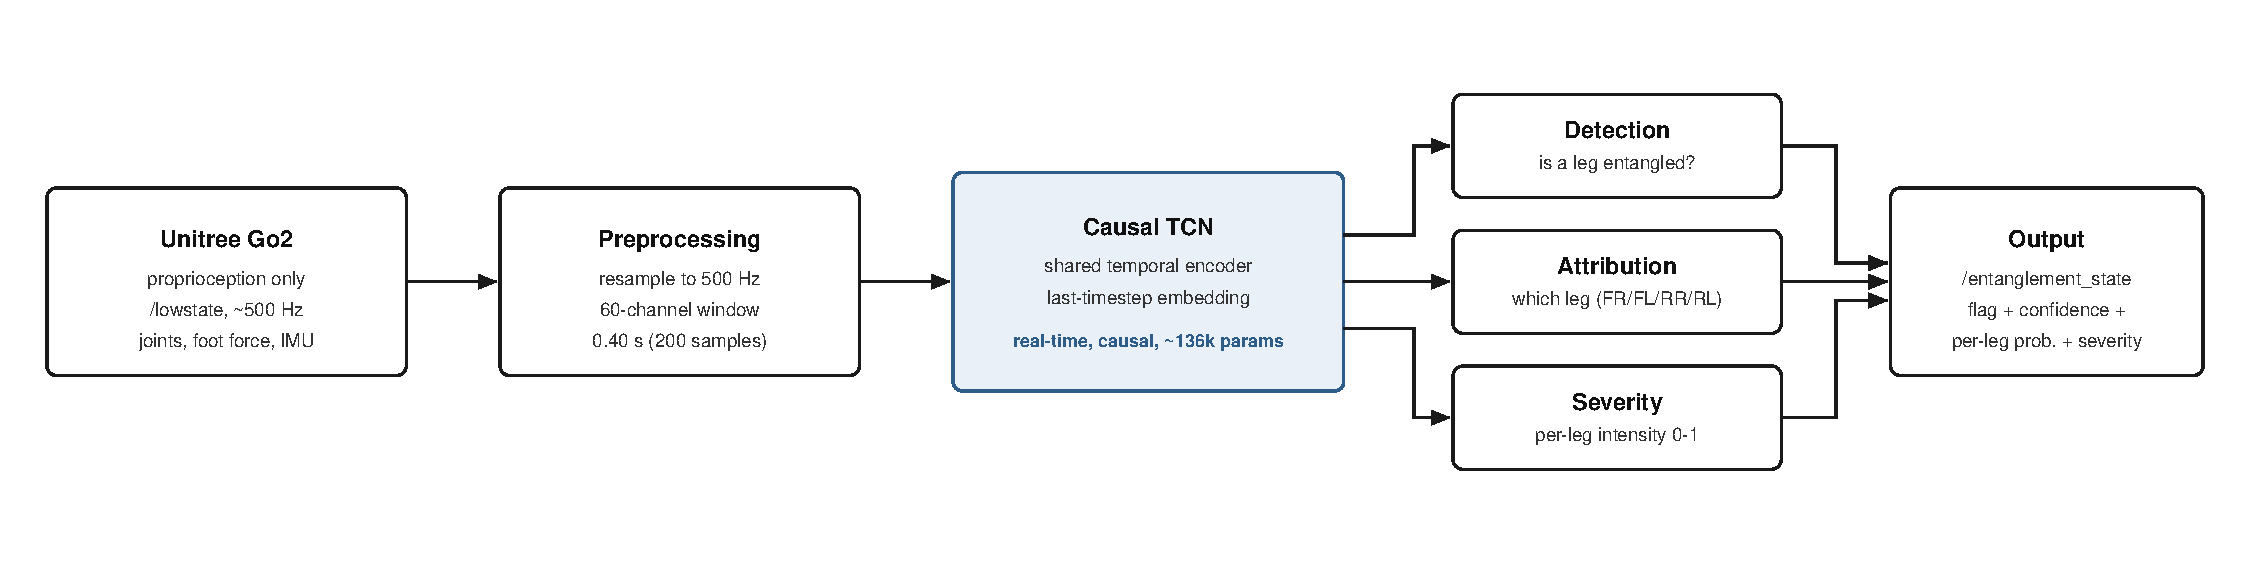
\includegraphics[width=\textwidth]{figures/fig1_system.pdf}
\caption{Overall system architecture. Proprioception from the Go2 is windowed and passed through a
shared causal TCN encoder whose three heads answer whether a leg is entangled, which leg, and how
severely; the result is published as a single state estimate.}
\label{fig:system}
\end{figure*}

\section{Related Work}

The work most directly comparable to ours is Yim et al.~\cite{yim2023entanglement}, which detects leg entanglement from proprioception and, when a leg becomes snagged, executes a disentanglement maneuver as that leg advances through its swing phase. Their system succeeds in 14 of 16 laboratory trials spanning obstacle stiffness and geometry, and it also holds up in outdoor tests, so entanglement is a real and tractable failure mode for legged locomotion. Detection and reaction are largely rule-based and reactive, coupled to gait-phase timing rather than to a learned temporal model, and the pipeline treats sensing and control as one loop. We keep the same proprioceptive premise but change three things. First, we integrate evidence over a fixed $0.40$~s window with a learned causal model instead of applying an instantaneous threshold, which lets brief resistive transients accumulate into a decision rather than trigger one immediately. Second, we produce structured outputs: which of the four legs is affected and a calibrated per-leg severity in $[0,1]$, rather than a single binary event. Third, we treat detection as a self-contained perception problem that consumes a published state estimate, so the detector is decoupled from any actuation policy. We do not claim our detector reacts faster or acts on the world; the contrast is in what is inferred and how it is reported, not in closing a control loop.

Learning from proprioception has become standard for legged control. Hwangbo et al.~\cite{hwangbo2019learning} and Lee et al.~\cite{lee2020learning} show that policies trained largely on joint and inertial signals transfer to hardware and cope with terrain that was never seen at training time, which establishes that proprioceptive streams carry enough information to reason about contact and disturbance. A related line estimates contact state and actuator faults from the same signals: Camurri et al.~\cite{camurri2017contact} infer foot contact probabilistically for state estimation, and Bledt et al.~\cite{bledt2018contact} detect contact events to inform gait. Entanglement differs from these in kind. A snag is an externally imposed kinematic constraint, applied at an unpredictable time and place, that resists a leg's intended motion without necessarily changing its nominal contact schedule. It therefore has to be localized to a specific leg and graded by how strongly it resists, which is what motivates our per-leg attribution and physics-grounded severity index rather than a single contact-versus-no-contact readout.

For the temporal model itself we build on temporal convolutional networks~\cite{bai2018tcn} and the dilated causal convolutions introduced for audio generation in WaveNet~\cite{oord2016wavenet}. A causal, dilated design fits streaming proprioception for two reasons. Causality means the prediction at each timestep uses only past and present samples, so the model can run online without waiting for future data. Dilation stacks a modest number of layers into a receptive field wide enough to span a stride, which lets the network relate the onset of resistance to its persistence over the window without the sequential dependency of a recurrent model. These properties, rather than raw capacity, are why the architecture suits an at-every-timestep detector on a mobile robot.

A detector is only usable if its confidence score can be turned into a threshold an operator trusts, which places probability calibration on the critical path. Modern networks are frequently over-confident, and post-hoc methods such as temperature scaling~\cite{guo2017calibration} and the earlier calibration analysis of Niculescu-Mizil and Caruana~\cite{niculescu2005predicting} recalibrate scores after training so that a reported probability better reflects an empirical frequency. We adopt temperature scaling in the same spirit, mainly to de-saturate probabilities that would otherwise pin near $1.0$ and force the operating threshold to an unusable extreme; we report its effect in full, including where it does not improve every calibration measure. This lets us choose an operating point deliberately rather than by inspecting a saturated score.

\section{Methodology}
\label{sec:method}
\subsection{Data Collection}

Our data come from a single Unitree Go2 quadruped, whose onboard proprioception is published on the ROS~2 topic \texttt{/lowstate}~\cite{macenski2022ros2,unitree_go2}. We recorded this stream while running a set of scripted locomotion scenarios, each designed to place the robot in a controlled situation and to log everything the joints, feet, and body sensors reported during it. Figure~\ref{fig:data} shows the collection pipeline end to end, from the live \texttt{/lowstate} messages through per-recording comma-separated-value (CSV) logs to the manually labeled dataset used for training and evaluation.

Each scripted scenario walks the robot for a while and, in the positive cases, drives one leg into a physical entanglement (for example, a wire or a hand snagging the limb) before releasing it. We also scripted purely negative scenarios that contain no entanglement at all, as well as a deliberate \texttt{Lock} condition: a rigid stance the robot holds immediately after standing up. \texttt{Lock} matters because it produces large, sustained joint torques with almost no motion, which superficially resembles a snag; including it as a scripted negative lets the model learn to tell a held stance apart from a genuine entanglement.

Logging is event-driven rather than clocked, so the effective sample rate is not uniform. Across recordings it ranges from roughly $410$ to $500$~Hz, with a median near $483$~Hz. We keep this raw, non-uniform timing in the recorded logs and defer resampling to the feature stage, so that no timing assumption is baked into the collected data.

The full corpus is $25$ recordings totaling $159{,}001$ labeled rows. Each row has $51$ columns, which fall into three sensor groups plus a label. The motor group holds $36$ values: the four legs, each with a hip, thigh, and calf joint, and for every joint a position $q$, a velocity $dq$, and a torque $\tau$. The next group is the four foot-contact forces, one per leg. The last sensor group is the inertial measurement unit (IMU), reporting body roll, pitch, and yaw, the three gyroscope axes, and the three accelerometer axes. A final \texttt{Status} column carries the phase label. Table~\ref{tab:dataset} summarizes these groups and the recording counts.

We labeled the recordings by hand. Because every scenario was scripted, we knew when an entanglement was induced and released, and we used those recorded timestamps together with per-joint torque plots to mark the exact rows spanning each event. The torque traces are the more reliable cue: a snagged limb shows a distinctive sustained resistive torque, which is visible in the plots even when the wall-clock timestamps drift slightly from the logged samples. Each row receives one of the phase labels \texttt{Walking}, \texttt{Entangled}, \texttt{Stop}, \texttt{Lock}, or blank, and the affected leg for a positive recording is encoded in that recording's filename.

Of the $25$ recordings, $15$ are positive (each containing one contiguous entangled event) and $10$ are negative. The positive events are not evenly distributed across the four legs. Grouping by the affected leg gives seven recordings for the rear-right leg, five for the rear-left, four for the front-left, and only three for the front-right. The front-right leg is therefore under-represented, and we flag it here because it constrains how confidently the per-leg behavior for that limb can be estimated; the effect resurfaces in the per-leg results (Figure~\ref{fig:perleg}). Figure~\ref{fig:dataset} plots the distribution of labels and per-leg positives across the dataset.

The way recordings are split into training, validation, and test sets is central to the credibility of every number we report, so we describe it before any modeling detail. We split at the level of whole recordings, assigning $16$ recordings to training, $4$ to validation, and $5$ to test, so that no recording contributes rows to more than one partition. The alternative, cutting the pooled rows or sliding windows at random, would be a mistake: consecutive windows from one recording overlap heavily and share the same robot, the same scripted scenario, and the same entanglement event, so a window in the test set would be nearly identical to windows the model trained on. That kind of window-level split leaks the answer and inflates the metrics. Grouping by recording forces the model to generalize to events it has never seen. The held-out test set is \texttt{back\_left\_hand2}, \texttt{back\_right\_wire1}, \texttt{front\_left\_hand2}, and \texttt{front\_both\_wire2} as positives, with \texttt{go2\_lowstate\_lock\_stop} as the negative, giving four positive recordings and one negative.
\begin{table}[t]
\centering
\caption{Dataset composition. 25 recordings, 159{,}001 labeled rows, logged non-uniformly
($\approx$410--500\,Hz, median $\approx$483\,Hz) and resampled to 500\,Hz at the feature stage. The
affected leg is encoded in the file name.}
\label{tab:dataset}
\footnotesize
\begin{tabular}{@{}lccl@{}}
\toprule
Scenario & \#Rec. & Affected & Interaction \\
\midrule
\texttt{back\_both}  & 2 & RR, RL & wire \\
\texttt{back\_left}  & 3 & RL     & hand / wire \\
\texttt{back\_right} & 3 & RR     & hand / wire \\
\texttt{front\_both} & 2 & FR, FL & wire \\
\texttt{front\_left} & 2 & FL     & hand \\
\texttt{front\_right}& 1 & FR     & wire \\
\texttt{back\_right} (at rest) & 2 & RR & wire \\
\midrule
\texttt{walking} & 5 & --- & normal gait \\
\texttt{stop}    & 3 & --- & standing \\
\texttt{lock\_stop}, \texttt{walk\_stop\_back} & 2 & --- & Lock / backward \\
\midrule
\textbf{Total} & \textbf{25} & \multicolumn{2}{l}{\textbf{15 positive / 10 negative}} \\
\bottomrule
\end{tabular}
\end{table}
\begin{figure*}[t]
\centering
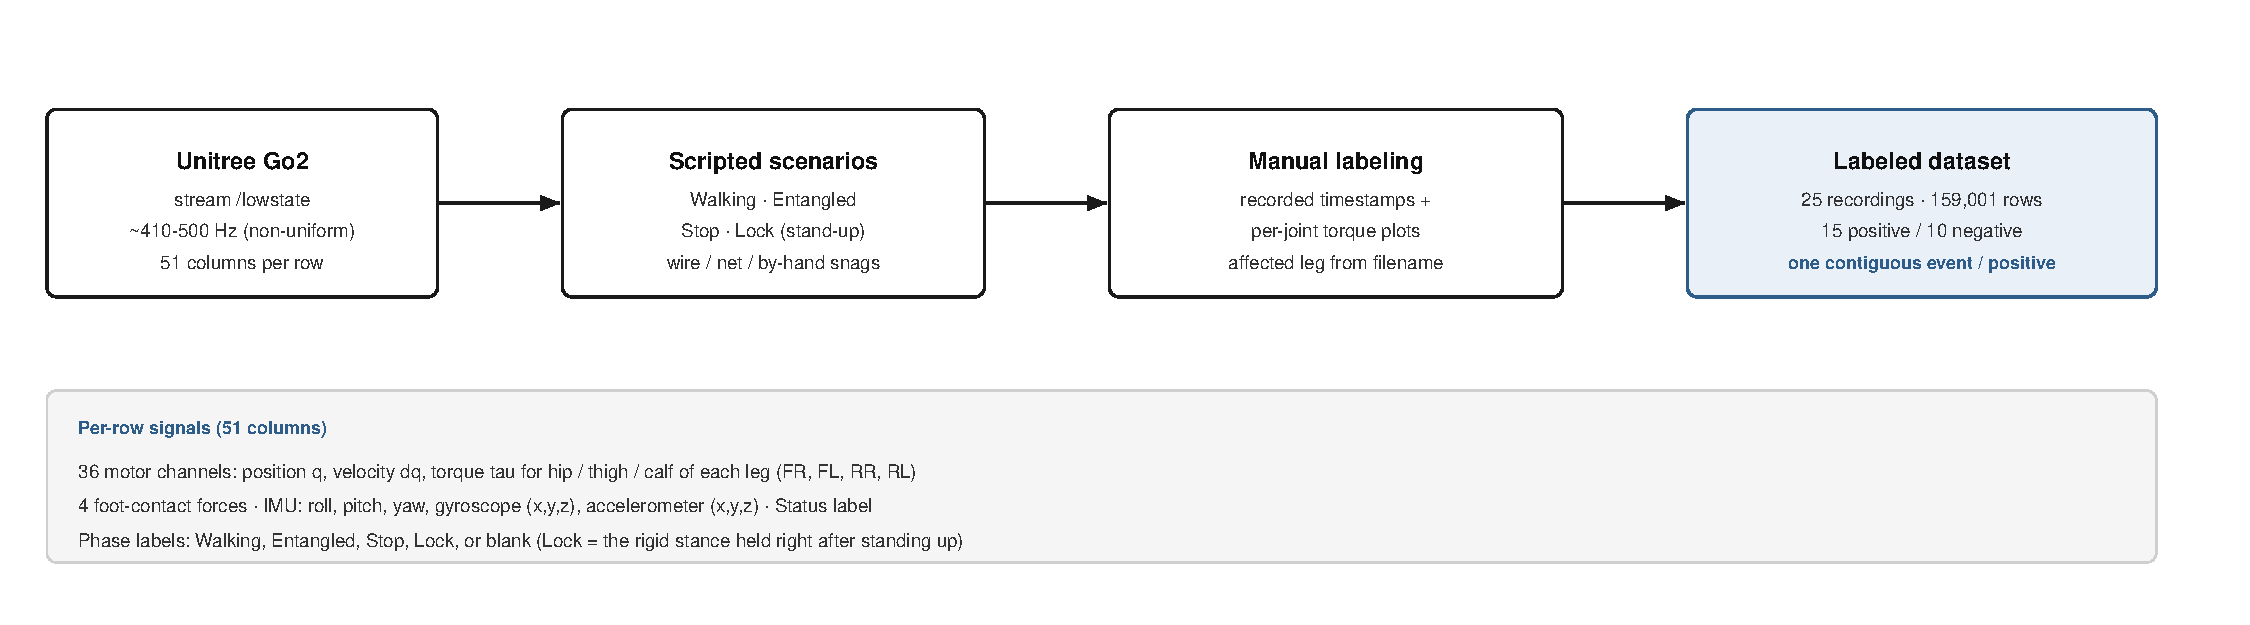
\includegraphics[width=\textwidth]{figures/fig2_data.pdf}
\caption{Data-collection pipeline. Scripted scenarios are streamed from \texttt{/lowstate}, labeled
manually from timestamps and per-joint torque plots, and grouped into a leakage-safe corpus.}
\label{fig:data}
\end{figure*}
\begin{figure*}[t]
\centering

\includegraphics[width=\textwidth]{figures/dataset_distribution.pdf}
\caption{Dataset distribution. (a) Positive recordings per affected leg; the front-right leg is
under-represented. (b) The leakage-safe split, grouped by whole recording.}
\label{fig:dataset}
\end{figure*}

\subsection{Feature Engineering}
\label{sec:feat}

Raw logs from the Go2 arrive at a non-uniform rate that varies from recording to recording, roughly 410 to 500~Hz with a median near 483~Hz. A temporal convolution assumes a fixed sampling interval: a filter of a given length always spans the same number of milliseconds, and dilations correspond to fixed time offsets. If we fed the network raw logs, a window of 200 samples would cover a different physical duration in each recording, and the learned filters would mean different things across files. We therefore resample every recording onto a common 500~Hz grid (a 2~ms step) before anything else. The continuous signals (joint positions, velocities, torques, foot forces, IMU) are resampled with linear interpolation, which is a reasonable model for smooth mechanical quantities. The \texttt{Status} label is categorical, so it is resampled with nearest-neighbor interpolation, which preserves the discrete phase identity of each row rather than blending two labels into a meaningless intermediate.

The resampled signal is turned into a 60-channel per-timestep representation, summarized in Table~\ref{tab:features} and sketched in Fig.~\ref{fig:feat}. Of these, 48 are raw sensor channels: the 36 motor channels (four legs, each with hip, thigh, and calf joints, each reporting position $q$, velocity $dq$, and torque $\tau$), the 4 foot-contact forces, and 8 of the IMU channels. We keep roll, pitch, the three gyroscope axes, and the three accelerometer axes, but drop yaw. Yaw is the integral of the yaw rate and has no fixed reference on level ground, so over a long recording it drifts as an unbounded integrator; feeding it to a normalizer would tie the features to an arbitrary starting heading.

The remaining 12 channels are engineered, three per leg, and they encode the mechanical signature we expect entanglement to produce. The intuition is simple. When a leg snags on a wire or a bar, the motor keeps commanding motion, but the limb cannot move, so the joint develops a large torque while its velocity stays near zero. A raw torque channel alone does not capture this, because a leg also produces large torques during normal, fast strides. What distinguishes a snag is torque \emph{in the resisting direction} combined with an absence of motion. The three per-leg features make that pattern explicit.

The first feature isolates the resistive component of the thigh torque, keeping only the downward (negative) part that opposes an upward pull:
\begin{equation}
\texttt{thigh\_tau\_down} = \max(0,\, -\tau_{\text{thigh}}).
\end{equation}
The second feature combines that resistive torque with the thigh velocity to express the ``high torque, little motion'' snag signature directly, using a small constant $\varepsilon = 0.05$ to keep the ratio finite when the leg is nearly still:
\begin{equation}
\texttt{thigh\_down\_effort} = \frac{\texttt{thigh\_tau\_down}}{|dq_{\text{thigh}}| + \varepsilon}.
\end{equation}
This ratio is large exactly when the thigh is pushing hard against a resistance while barely moving, which is the condition we care about, and small during ordinary swinging where velocity is high. The third feature sums the absolute torque across the leg's three joints,
\begin{equation}
\texttt{tau\_sum} = \sum_{j \in \{\text{hip},\,\text{thigh},\,\text{calf}\}} |\tau_j|,
\end{equation}
giving a scalar measure of total effort in that leg. Because it is computed per leg, it helps the model attribute an event to the correct limb rather than merely detecting that \emph{something} is stuck.

All 60 channels are then standardized by z-score normalization. The mean and standard deviation for each channel are estimated on training rows only, never on validation or test rows, so no information about the held-out recordings can leak into the normalization statistics.

The final step is windowing. The network reads a sliding window of 200 consecutive samples, which at 500~Hz is 0.40~s, approximately the duration of one trot stride. A window shorter than a stride could mistake the normal high-torque phase of a step for a snag, whereas one full stride gives the model enough context to tell a passing torque spike from a sustained resistance. During training we advance the window by a hop of 25 samples, which gives many overlapping examples while keeping them decorrelated; for evaluation we use a dense hop of 1 so that every timestep produces a prediction, matching how the detector runs online. A window is labeled positive when at least 50\% of its rows are marked \texttt{Entangled}. Windows in the ambiguous band, where the entangled fraction falls between 0.2 and 0.5, are excluded from training so the classifier learns from clean examples, but they are retained for evaluation so the reported metrics reflect the harder, realistic transitions. Windows dominated by the \texttt{Stop} or \texttt{Lock} phases are treated as negatives.
\begin{table}[t]
\centering
\caption{The 60-channel input representation. Motor torque is the estimated joint torque $\tau$.}
\label{tab:features}
\footnotesize
\begin{tabular}{@{}llc@{}}
\toprule
Group & Channels & Count \\
\midrule
Motor & 4 legs $\times$ \{hip, thigh, calf\} $\times$ \{$q,\dot q,\tau$\} & 36 \\
Foot force & one per leg & 4 \\
IMU & roll, pitch, gyro$_{xyz}$, acc$_{xyz}$ (yaw dropped) & 8 \\
Engineered & per leg: 3 physics features (Sec.~\ref{sec:feat}) & 12 \\
\midrule
\textbf{Total} & & \textbf{60} \\
\bottomrule
\end{tabular}
\end{table}
\begin{figure*}[t]
\centering
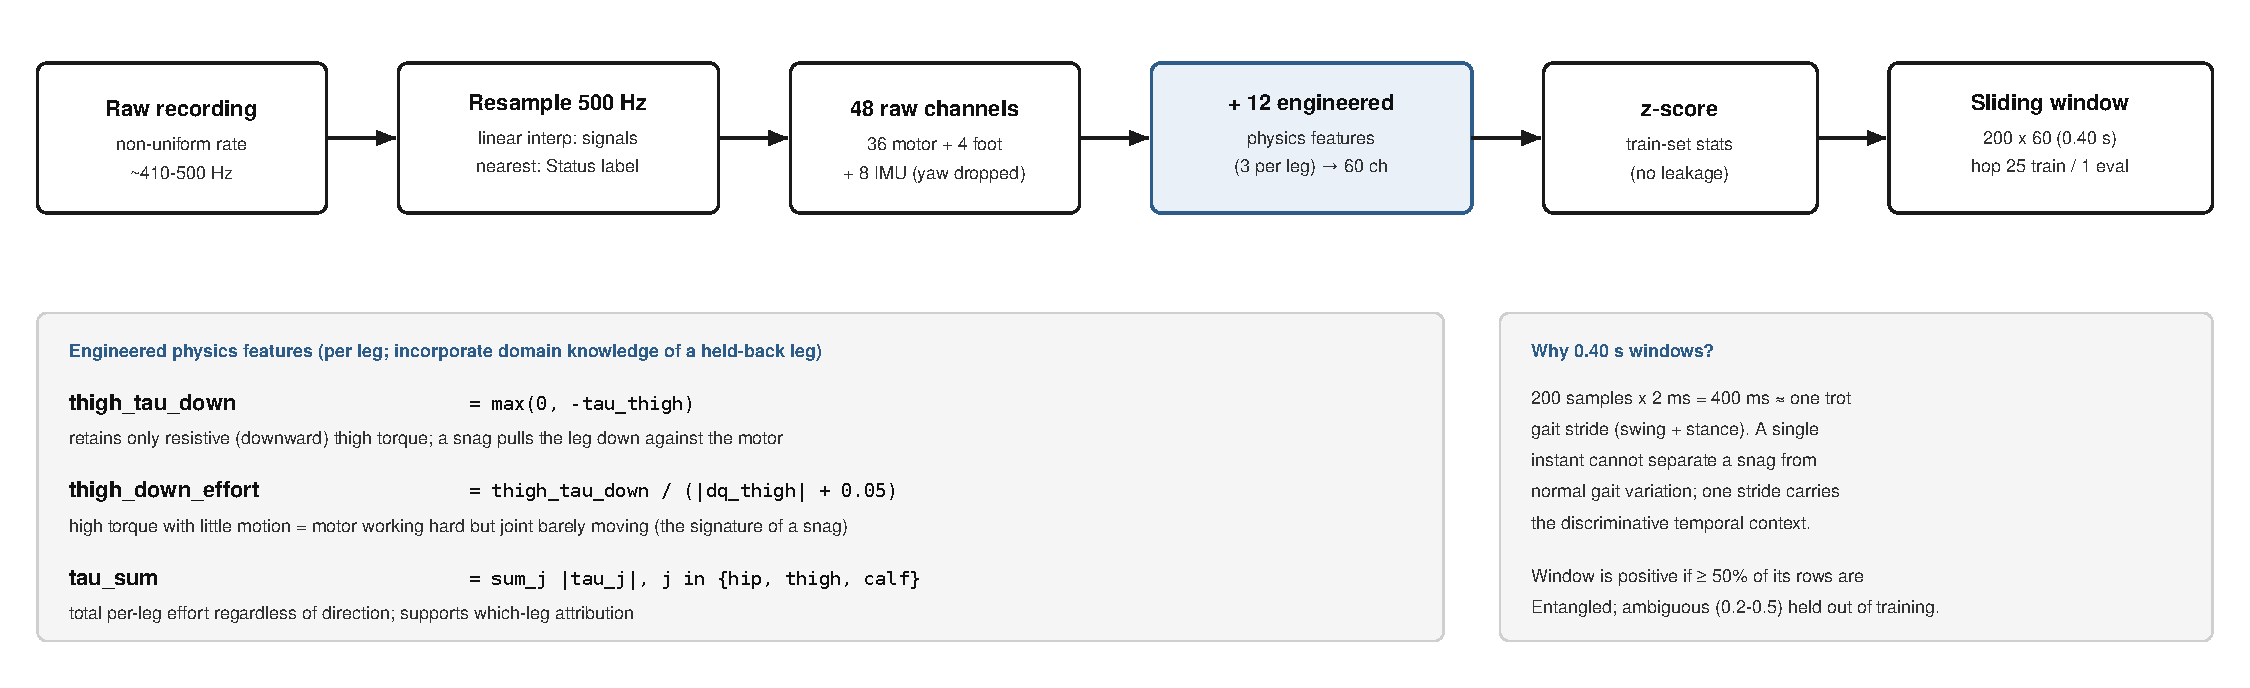
\includegraphics[width=\textwidth]{figures/fig3_features.pdf}
\caption{Feature-engineering pipeline. Recordings are resampled to a common 500\,Hz, expanded to 60
channels (48 raw + 12 engineered physics features), normalized with training statistics, and cut
into overlapping 0.40\,s windows.}
\label{fig:feat}
\end{figure*}

\subsection{Machine Learning Pipeline}

Every 0.40\,s window (200 samples at 500\,Hz, 60 channels) must yield three answers at once: is any leg entangled, which leg, and how severe. A model built for this has to respect one hard operational constraint. At inference the detector sees a stream that ends at the current instant and can never peek ahead, so the network must produce, at time $t$, a decision that depends only on samples up to and including $t$. We use a temporal convolutional network (TCN) \cite{bai2018tcn} because it satisfies this constraint by construction, processes a whole window in parallel rather than one step at a time, and grows its temporal reach cheaply through dilation. The architecture is shown in Fig.~\ref{fig:tcn}, and its hyperparameters are collected in Table~\ref{tab:hparams}.

Causality is enforced through left-padding. A standard convolution centred on $t$ mixes in future samples; instead we pad only the left (past) side of each sequence so that the output at $t$ is a function of $\{x_{t-k},\dots,x_t\}$ and nothing later. The immediate benefit is that the model we train offline on complete recorded windows is numerically the same function that runs online on a growing buffer: there is no train-test discrepancy from windowing or look-ahead, a property we verify empirically later. This mirrors the causal-convolution idea from WaveNet \cite{oord2016wavenet}, adapted here to multivariate proprioception rather than audio.

The input first passes through a causal convolutional stem that lifts the 60 input channels to a 64-dimensional feature space, giving the residual stack a consistent width to operate on. Five residual blocks follow, with dilation factors $1,2,4,8,16$. Dilation inserts gaps between the taps of a kernel so that a fixed kernel size covers an exponentially longer span as we stack blocks, which is how a small network reaches far back in time without a matching blow-up in parameters or compute. With kernel size 3 and these five dilations, the receptive field is 127 samples, or 254\,ms at 500\,Hz. That is comfortably inside the 0.40\,s window, so the last output position has actually seen most of a trot stride before it commits to a decision.

Each residual block has the same internals: a causal convolution, a GELU nonlinearity \cite{hendrycks2016gelu}, a second causal convolution, another GELU, dropout at rate 0.1, and then an identity skip connection that adds the block input back to its output. The skip connection lets gradients flow past the block and makes each block learn a refinement of its input rather than a full remapping, which stabilises training of the stack. Both convolutions use weight normalization \cite{salimans2016weightnorm}, which decouples the scale of each filter from its direction and tends to smooth optimization. GELU is a smooth gating nonlinearity that we found preferable to a hard rectifier for these continuous torque and velocity signals.

After the stack we read out only the embedding at the last timestep, a single 64-dimensional vector. This is deliberate: at deployment the quantity of interest is the decision \emph{now}, given the history in the buffer, and the last position is precisely the one whose receptive field ends at the present sample. That 64-D readout feeds three linear heads. The detection head emits one logit (entangled or not). The leg head emits four logits, treated as independent labels because more than one leg can be affected. The intensity head emits four values, one per leg. The whole network has 136{,}393 parameters, roughly 136k, small enough to ship as a half-megabyte model.

The three tasks are trained jointly with a single weighted objective. Detection and leg attribution are classification problems and use binary cross-entropy; intensity regression uses a Huber loss, which behaves like squared error for small residuals but like absolute error for large ones and so is less swayed by outliers. Detection and leg are weighted equally, and the intensity term is down-weighted because it is an auxiliary signal, not a headline output. In words, the loss is one part detection cross-entropy, one part leg cross-entropy, and three-tenths of a part intensity Huber:
\begin{equation}
\mathcal{L} = 1.0\,\mathrm{BCE}_{\text{det}} + 1.0\,\mathrm{BCE}_{\text{leg}} + 0.3\,\mathrm{Huber}_{\text{int}} .
\end{equation}
The intensity term deserves a caveat. Its Huber ($\delta=0.1$) is computed against a physics pseudo-target, not a human-labeled severity, and elements corresponding to the affected leg are up-weighted $3{:}1$ relative to the rest. This is an up-weight, not a hard mask: because most legs at most times carry a target of zero, leaving the weighting flat would let ``predict zero everywhere'' dominate the loss and the head would learn nothing about the affected leg. The head therefore ends up as a weak learner that tracks the physics target, while the physics formula itself remains authoritative at inference.

Two further measures handle the strong class imbalance between normal and entangled windows. A class-balanced weighted sampler equalises exposure to positives and negatives during training, and each classification task carries a (capped) positive-class weight in its cross-entropy. Optimization uses AdamW \cite{loshchilov2019adamw} with a cosine-annealed learning rate over 30 epochs; the exact learning rate, weight decay, batch size, and seed are listed in Table~\ref{tab:hparams}.

Severity is reported through a physics-grounded index rather than the network head alone, because no ground-truth severity labels exist to regress against. The index combines three quantities per leg. A confidence gate $g$ is the per-leg entanglement probability, so the index is near zero whenever the leg is not flagged and cannot manufacture severity out of noise. A deviation term $d$ is the Mahalanobis distance of the window's per-leg feature vector from the normal walking distribution (mean and covariance fit on training walking data only), measuring how far the leg's kinematics have drifted from ordinary gait. A resistive-effort term $r$ is the mean of the downward thigh torque divided by thigh joint speed, high when a leg pushes hard yet barely moves, the signature of a snag. These combine as
\begin{equation}
I_{\text{leg}} = g\,\sqrt{d\,r},
\end{equation}
with the square root compressing the product of deviation and effort, and the result calibrated to $[0,1]$. Because there is no severity ground truth, we present $I_{\text{leg}}$ as a calibrated index, not a measured force. The value deployed to the runtime blends the network head and this physics index in equal parts, so learned evidence and analytic evidence are given the same say.

The choice of a TCN over the obvious alternatives follows from these requirements. A recurrent network is sequential and awkward to make strictly causal-equivalent between offline and online use, and it trains one step at a time; the TCN is causal by padding, evaluates a window in parallel, and reaches 254\,ms of history for a small parameter budget. A gradient-boosted tree ensemble, though a strong tabular baseline, has no native notion of time and would have to be handed hand-built window summaries, discarding exactly the temporal structure that distinguishes a transient snag from a steady stance.
\begin{figure*}[t]
\centering
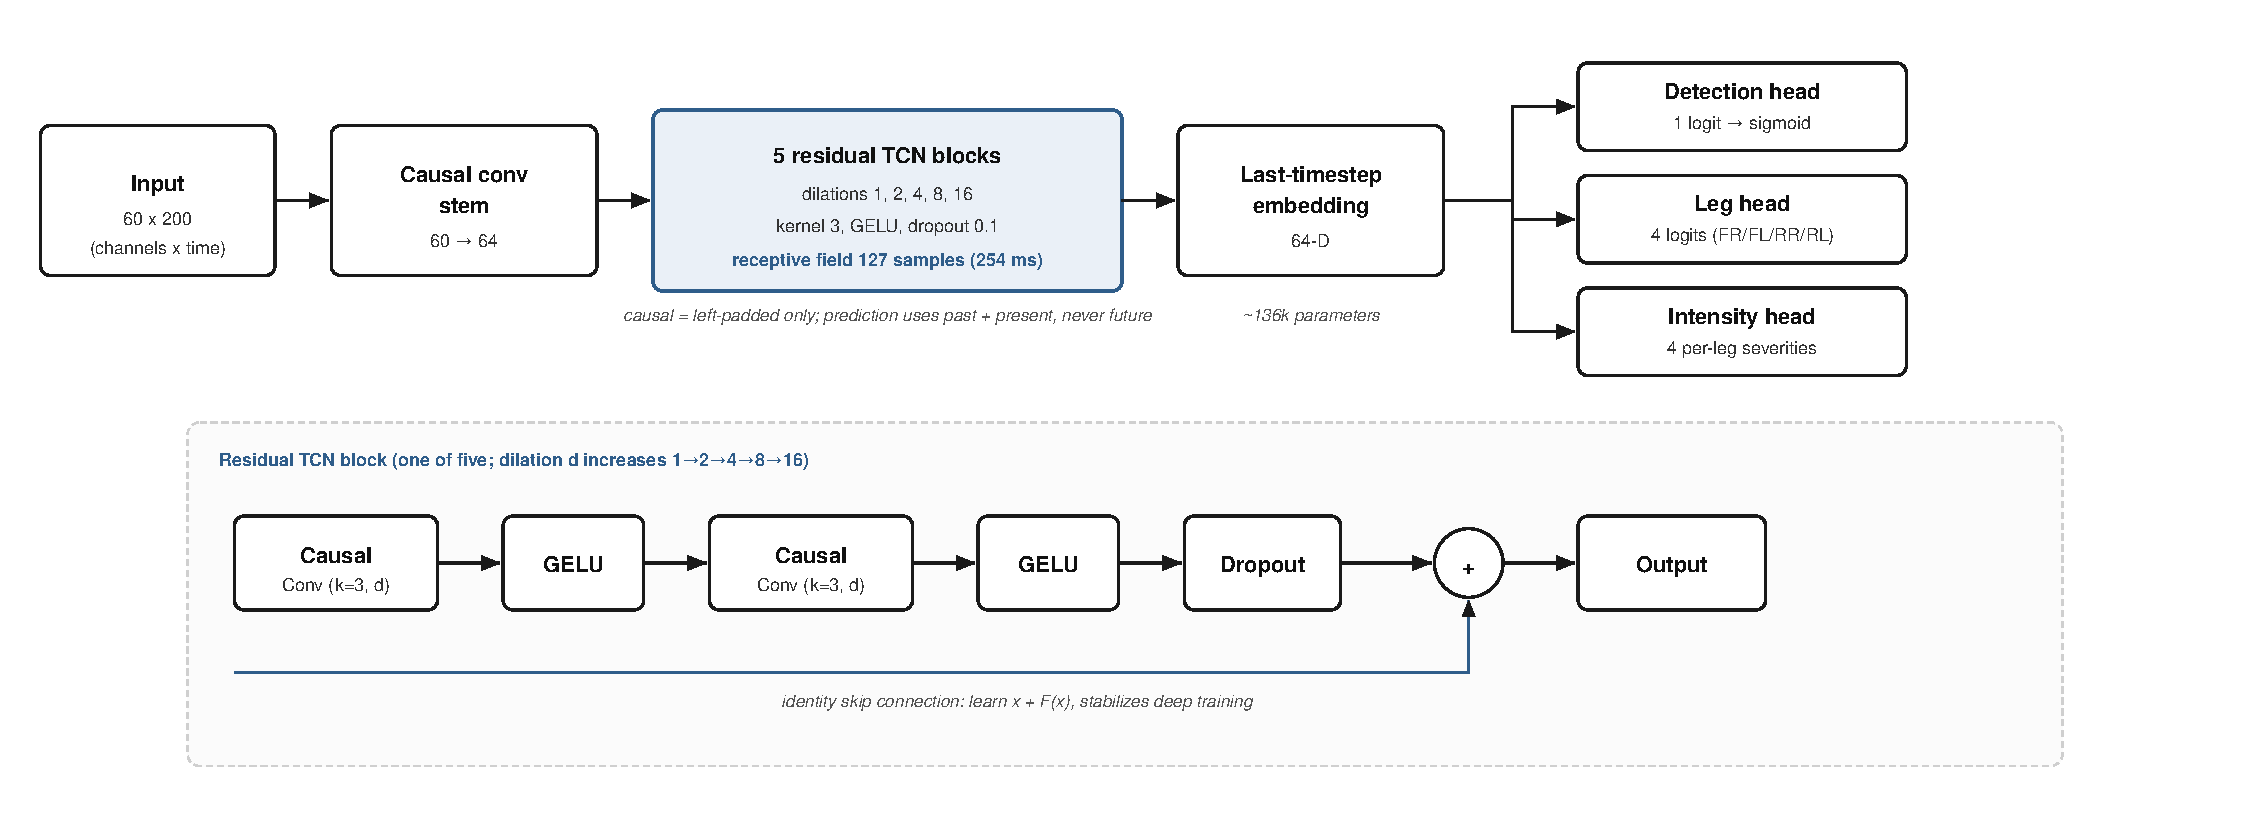
\includegraphics[width=\textwidth]{figures/fig4_tcn.pdf}
\caption{Multi-task causal TCN. A causal convolutional stem feeds five dilated residual blocks; the
last-timestep 64-D embedding drives the detection, leg-attribution, and intensity heads. The inset
shows one residual block.}
\label{fig:tcn}
\end{figure*}
\begin{table}[t]
\centering
\caption{Model and training configuration.}
\label{tab:hparams}
\footnotesize
\begin{tabular}{@{}ll@{}}
\toprule
Item & Value \\
\midrule
Window / hop (train, eval) & 200 (0.40\,s) / 25, 1 \\
Resample rate & 500\,Hz \\
Encoder width / blocks & 64 / 5 \\
Dilations; kernel; dropout & 1,2,4,8,16; 3; 0.1 \\
Receptive field & 127 samples (254\,ms) \\
Parameters & 136{,}393 \\
Loss weights (det / leg / int.) & 1.0 / 1.0 / 0.3 \\
Intensity Huber & $\delta{=}0.1$, affected-leg $3{:}1$ up-weight \\
Optimizer & AdamW, lr $10^{-3}$, wd $10^{-4}$ \\
Schedule; batch; epochs; seed & cosine; 256; 30; 1234 \\
Sampler & class-balanced, rare-leg up-weighted \\
\bottomrule
\end{tabular}
\end{table}

\subsection{Runtime Architecture}
\label{sec:runtime}

On the robot the detector is a ROS~2 node that turns the raw telemetry stream into a published
state estimate. Figure~\ref{fig:runtime} shows its internal path, and Figure~\ref{fig:e2e} places
that path in the larger picture: the same preprocessing and model serve offline training and online
inference, and only the exported ONNX model together with the saved normalization and calibration
statistics cross the deploy boundary.

The node subscribes to \texttt{/lowstate} with \texttt{BEST\_EFFORT} quality of service. Reliable
delivery would add retransmission latency to a stream that arrives hundreds of times per second, and
a dropped proprioceptive sample matters far less than a late one, so trading guaranteed delivery for
low latency is the right call. Each message is adapted into the 48 raw signals the model expects and
pushed into a 200-sample circular ring buffer; the buffer holds memory and per-sample cost constant,
since the oldest sample is overwritten as each new one arrives rather than reallocating a growing
window. Once the buffer is full it is expanded to the 60-channel representation and normalized with
the statistics saved at training time.

Inference runs through ONNX Runtime rather than PyTorch. The exported graph loads faster, uses less
memory, and removes the training-framework dependency from the robot, which matters on a constrained
onboard target~\cite{onnxruntime,macenski2022ros2}. The detection logit is passed through a sigmoid
and, separately, through a temperature-scaled sigmoid ($T=5.918$) to produce the reported confidence;
the per-leg severity is the equal-weight blend of the network head and the physics index. Raw network
predictions flicker from sample to sample, so a detection is latched only after the raw probability
stays above threshold for 75~ms. That short temporal debounce suppresses isolated spikes without
noticeably delaying a genuine alarm. Per-leg thresholds then name the affected leg, with the
rear-right threshold raised to 0.9 because that leg was the most prone to false positives; the others
use 0.5. Operating-point values are collected in Table~\ref{tab:oppoint}. The node publishes
\texttt{/entanglement\_state}, carrying the debounced flag, the calibrated confidence, four per-leg
probabilities, four per-leg severities, and the name of the alarm leg.

\subsubsection{Stationarity gate}
One failure mode surfaced only in testing. When the robot walks, stops, and then stiffens into the
rigid Lock stance it holds after standing up, the ring buffer still contains the tail of the walking
motion, and the detector can briefly report entanglement for a robot that is simply standing still.
The gate that fixes this watches the mean absolute joint velocity: when it falls below 0.30~rad/s for
100~ms the robot is treated as stationary, and the node clears the ring buffer, resets the debounce
counter, and arms a 300~ms suppression window that ignores the transient while gait is re-acquired.
The gate is edge-triggered, so it acts once on the transition rather than continuously. It is disabled
in the research configuration so that the evaluation pipeline is byte-identical to the deployed one,
and enabled only on the robot.
\begin{figure*}[t]
\centering
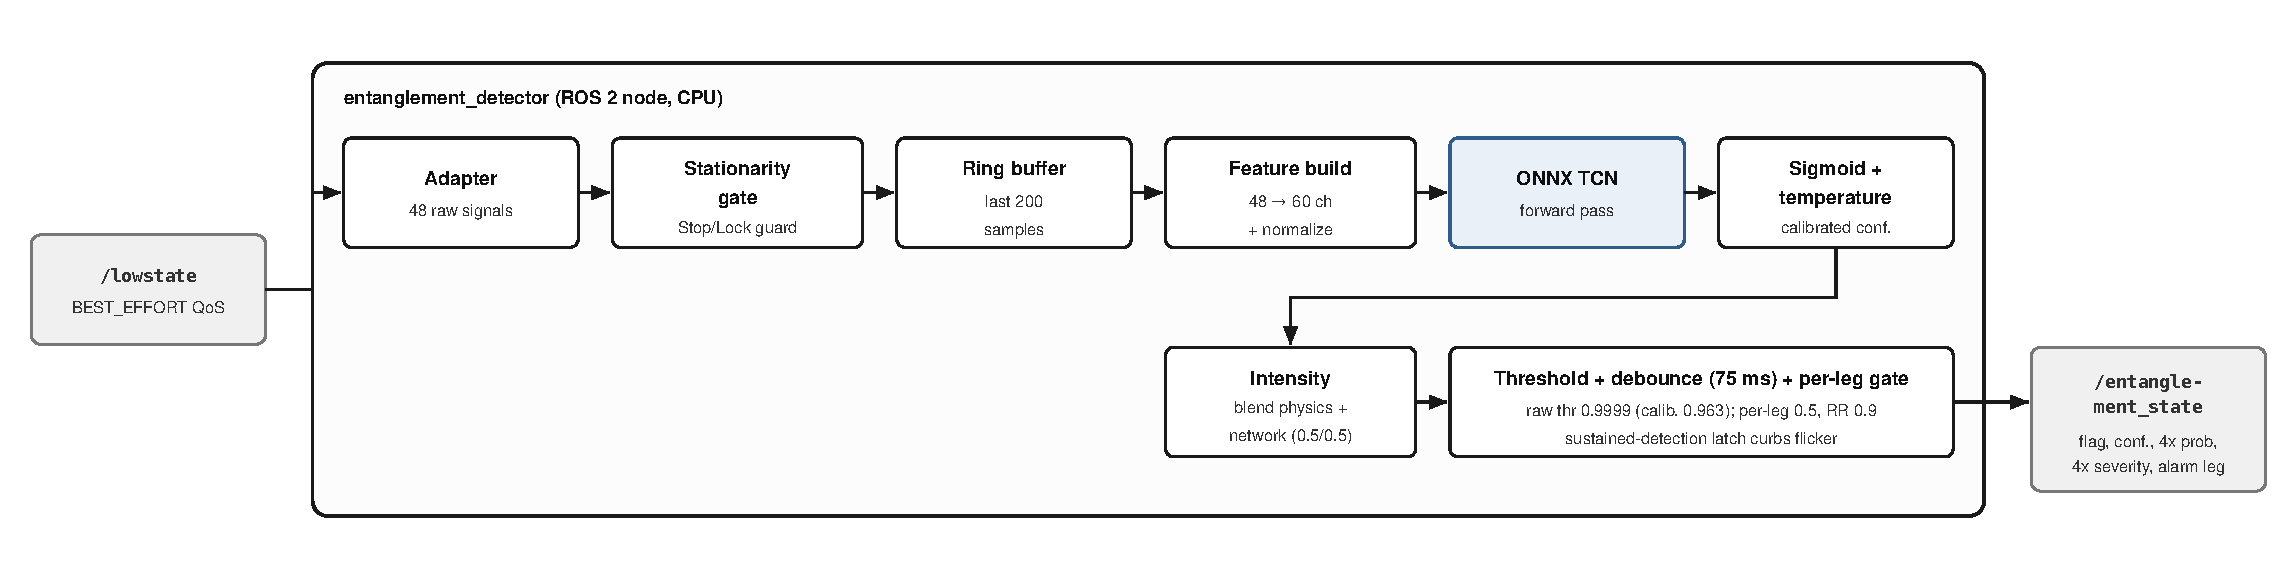
\includegraphics[width=\textwidth]{figures/fig5_runtime.pdf}
\caption{On-robot ROS\,2 runtime. The \texttt{entanglement\_detector} node maintains a ring buffer,
runs ONNX inference, and applies calibration, debouncing, per-leg thresholds, and a stationarity gate
before publishing \texttt{/entanglement\_state}.}
\label{fig:runtime}
\end{figure*}
\begin{table}[t]
\centering
\caption{Deployment operating point (all post-hoc; the trained weights are unchanged).}
\label{tab:oppoint}
\footnotesize
\begin{tabular}{@{}ll@{}}
\toprule
Item & Value \\
\midrule
Backend & ONNX Runtime, CPU \\
Input QoS & \texttt{BEST\_EFFORT} \\
Temperature $T$ & 5.918 \\
Detection threshold (raw / calibrated) & 0.9999 / 0.963 \\
Debounce & 75\,ms \\
Per-leg thresholds & FR/FL/RL $=0.5$; RR $=0.9$ \\
Intensity blend (network / physics) & 0.5 / 0.5 \\
Stationarity gate & $|\dot q|<0.30$\,rad/s for 100\,ms \\
\bottomrule
\end{tabular}
\end{table}
\begin{figure*}[t]
\centering
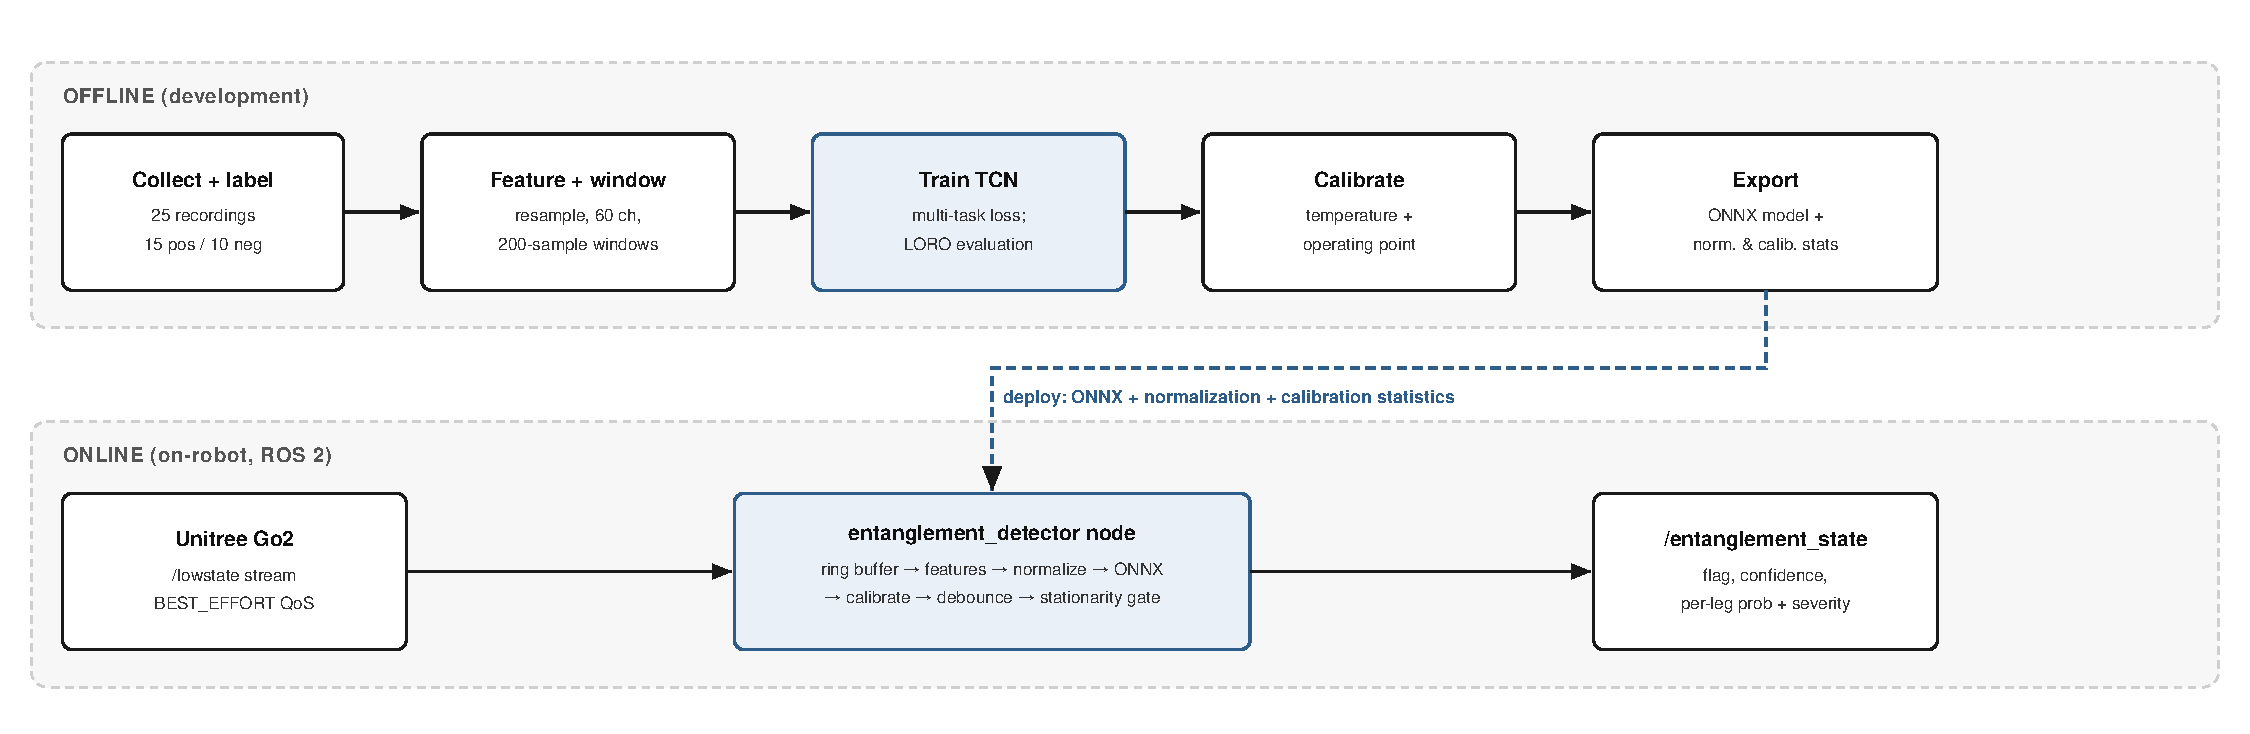
\includegraphics[width=\textwidth]{figures/fig6_endtoend.pdf}
\caption{End-to-end pipeline. The same preprocessing and model are used offline for training and
online for inference; only the exported ONNX model and the saved normalization and calibration
statistics cross the deploy boundary.}
\label{fig:e2e}
\end{figure*}

\section{Experimental Setup}
Evaluation choices for this problem are dominated by one fact: entanglements are rare, contiguous events, and the 25 recordings differ in gait, terrain contact, and which leg is affected. A window-level random split would place windows from the same recording on both sides of the partition, and because neighboring windows share almost all of their samples, that arrangement leaks information and inflates every score. All protocols below therefore group by whole recording so that no recording contributes to both training and test.

\subsection{Data splits}
We report two complementary protocols. The first is a fixed leakage-safe split, grouped at the recording level, of 16 training / 4 validation / 5 test recordings; the five test recordings (four positive, one negative) are held out entirely and used only for the final numbers. Normalization statistics and the Walking reference distribution used by the physics severity index are fit on training rows alone, so no test information reaches the model or the feature pipeline.

The fixed split gives a single, interpretable operating-point result, but with 15 positive recordings any one test partition samples only a handful of events, and the affected legs are unevenly represented (FR appears in only three positive recordings). To measure generalization across recordings rather than across an arbitrary partition, we adopt leave-one-recording-out (LORO) cross-validation over the 15 positive recordings as the headline protocol: each fold holds out one positive recording, trains on the rest (with the negatives available for training), and evaluates on the held-out recording, and we report the mean and standard deviation of the per-fold $F_1$. LORO is the fairer test of whether the detector transfers to an event it has never seen, and its variance across folds is itself informative.

\subsection{Dense evaluation and metrics}
Training uses a stride of 25 samples between windows for efficiency, but evaluation is dense: we slide the 200-sample window with hop 1 so that a decision is produced at every timestep, matching how the runtime consumes \texttt{/lowstate}. This is the strictest setting, since it scores the boundaries of an event where the window straddles the transition into and out of the entangled phase.

We use standard definitions, each computed on the dense windows. Precision is the fraction of flagged windows that are truly entangled, recall the fraction of entangled windows that are flagged, and $F_1$ their harmonic mean. PR-AUC is the area under the precision--recall curve and ROC-AUC the area under the receiver-operating curve, both threshold-free summaries of the binary detection head; PR-AUC is the more meaningful of the two here because the positive class is rare. For the per-leg attribution task we report multi-label exact-match: a window counts as correct only when the predicted set of entangled legs equals the true set exactly, which is a deliberately unforgiving criterion.

\subsection{Rule-based baseline}
Snagged legs resist downward thigh motion, and a natural non-learned detector fires when the resistive thigh torque of any leg is high. We implement this thigh-torque heuristic and evaluate it under the identical dense, grouped protocol, on the same windows and the same test recordings, so the comparison in Table~\ref{tab:detection} isolates the value of the learned model rather than any difference in how the data are prepared.

\subsection{Feature ablation}
The shipped model reads 60 channels: 48 raw signals and 12 engineered per-leg features. To attribute performance to feature groups rather than infer it, we retrain the full model from scratch on channel subsets and re-run LORO for each: engineered features only (12), raw signals only (48), raw plus engineered without the foot-contact channels (56), raw plus engineered without the IMU channels (52), and the full 60-channel set. Because each variant is retrained under the same protocol, Table~\ref{tab:ablation} reflects the marginal contribution of each group under LORO variance rather than a post-hoc feature-importance estimate.

\subsection{Calibration}
The detector emits a probability, and downstream thresholding and debouncing behave well only if that probability is meaningful. We assess calibration in three ways. Brier score measures the mean squared error of the probabilities against the binary outcomes, expected calibration error (ECE) measures the gap between confidence and accuracy across probability bins, and we additionally inspect saturation, the fraction of raw probabilities pinned near 1.0. Saturation is the practical motivation here: when a large share of probabilities sit at the ceiling, the false-alarm-rate threshold is forced to an extreme value, and temperature scaling \cite{guo2017calibration,niculescu2005predicting} is applied to de-saturate the output so that a usable operating threshold exists. We report Brier, ECE, and saturation before and after scaling, without assuming that de-saturation implies better reliability.

\subsection{Latency}
Because the detector must keep pace with the 500 Hz feature stream, we benchmark inference time. Latency is measured on the deployment ONNX Runtime \cite{onnxruntime}, pinned to a single CPU thread, timing the per-window forward pass together with the post-processing (sigmoid, temperature scaling, threshold, and debounce logic) rather than the network alone. We report mean, median, and 95th-percentile per-window latency against the 2.0 ms budget implied by the sample step. This is a benchmark of the deployment runtime on a development CPU; it is not measured on the Go2's onboard computer, and we present it as such.

\section{Results}

We evaluate detection quality on the held-out test split, generalization across recordings, per-leg attribution, probability calibration, feature importance, deployment robustness, and runtime cost. Unless stated otherwise, every number reported here comes from offline replay of recorded logs; we make no claim about live on-robot detection performance.

\subsection{Detection on the held-out test split}
Our first question is whether the model separates entangled windows from everything else better than a hand-tuned heuristic operating on the same signal. Table~\ref{tab:detection} compares the TCN against a rule-based baseline that thresholds thigh torque, evaluated under an identical protocol on the same five test recordings. On the test split the TCN reaches precision $0.799$, recall $0.818$, and $F1 = 0.809$, with $\text{PR-AUC} = 0.808$ and $\text{ROC-AUC} = 0.956$. The rule-based baseline attains comparable precision ($0.735$) but collapses on recall ($0.131$), for $F1 = 0.222$; a fixed torque threshold catches only the most violent snags and misses the many entanglements that manifest as sustained resistive effort rather than a single large spike. The gap in $F1$ ($0.809$ vs.\ $0.222$) and in exact-match multi-label accuracy ($0.908$ vs.\ $0.106$) is the central detection result.

The confusion matrix in Fig.~\ref{fig:confusion} makes the error profile concrete at the operating point (raw threshold $0.9999$): TP $2833$, FP $712$, FN $630$, TN $9126$. Errors are roughly balanced between false alarms and misses, and the large true-negative count reflects the dominance of ordinary walking and stationary windows in the data.

Because a single threshold hides how the score behaves across all thresholds, Fig.~\ref{fig:rocpr} plots the full ROC and precision-recall curves. The ROC-AUC of $0.956$ indicates strong ranking of positive over negative windows; the lower PR-AUC of $0.808$ is expected under class imbalance, where precision is sensitive to the many negatives.

\subsection{Generalization across recordings (LORO)}
Test-split numbers depend on one particular grouping of recordings, so we also run leave-one-recording-out (LORO) cross-validation, which retrains with each recording held out in turn. Across the 15 folds shown in Fig.~\ref{fig:loro}, $F1 = 0.807 \pm 0.142$. The mean tracks the test-split $F1$ closely, which suggests the split is representative rather than lucky. The spread is not uniform: the weakest folds are the front-right recording, the least represented leg, together with the deployment recordings that capture entanglement while the robot stands at rest, a regime that differs most from the walking-dominated remainder of the corpus.

\subsection{Per-leg attribution}
Detecting that \emph{some} leg is entangled is only half the task; the system must also name the leg. Fig.~\ref{fig:perleg} and Table~\ref{tab:perleg} report per-leg detection on the test split. Recall is high across all four legs (FR $1.000$, FL $1.000$, RR $0.959$, RL $0.916$), so genuine entanglements are rarely missed regardless of which leg is involved. The differences live in precision. Front-right shows a clear precision/recall trade-off: it recovers every front-right event (recall $1.000$) but at precision $0.467$, giving $F1 = 0.636$, the lowest of the four. This is consistent with the LORO finding, since FR has the fewest positive appearances and the model compensates by firing readily on FR. The other legs are stronger: FL $F1 = 0.845$ (P $0.731$, R $1.000$), RL $F1 = 0.823$ (P $0.748$, R $0.916$), and RR $F1 = 0.700$ (P $0.551$, R $0.959$).

\subsection{Calibration}
A detector that outputs probabilities should ideally have those probabilities mean what they say. Fig.~\ref{fig:reliability} reports the reliability diagram before and after temperature scaling. The raw network is badly over-confident: roughly $27\%$ of window probabilities are pinned near $1.0$, and this saturation forces the false-alarm-controlled threshold to clamp at $0.9999$. Temperature scaling with $T = 5.918$ de-saturates the probabilities and lets the operating threshold move to a more usable $0.963$. The effect on scoring metrics is mixed: the Brier score improves slightly, from $0.128$ to $0.118$, but the expected calibration error does \emph{not} improve, moving from $0.134$ to $0.156$. Temperature scaling here buys us a de-clamped, interpretable threshold and a marginally better Brier score, not better calibration in the ECE sense.

\subsection{Feature ablation}
To understand which input channels carry the signal, we retrain with feature groups removed and re-run LORO for each configuration. Table~\ref{tab:ablation} and Fig.~\ref{fig:ablation} report the change in F1 relative to the full 60-channel set. Raw kinematics are essential: using the engineered channels alone drops F1 by $0.13$, and removing all raw channels is by far the largest degradation. The engineered channels still earn their place, since raw-only sits $0.03$ below the full set. Foot contacts matter little (removing them costs $0.01$) and the IMU is effectively redundant for this task: dropping it leaves F1 unchanged to two decimals. In short, joint position, velocity, and torque do the work, the engineered snag-signature channels add a small margin, and the inertial channels contribute almost nothing.

\subsection{Deployment robustness}
Offline test metrics do not capture failure modes that appear on specific field recordings, so we retrained with targeted data augmentation and measured per-phase firing rates before (v1) and after (v2) on the relevant recordings; Fig.~\ref{fig:field} summarizes these. Four false-fire modes were driven to essentially zero: the Lock false-fire on \texttt{lock\_stop} ($0.8 \to 0.0$) and on \texttt{walk\_stop\_back}-Lock ($4.7 \to 0.0$), rear-right firing while stopped on \texttt{back\_right\_intensity}-Lock ($100 \to 0$), and backward-walking firing on \texttt{walk\_stop\_back}-Walking ($9.7 \to 0$). On the front-right event (\texttt{front\_right\_wire}), binary firing rose from $30.7\%$ to $78.5\%$ and correct-leg firing rose from $4\%$ to $100\%$. This specialization was not free: adding the hard-negative Lock and backward-walking recordings cost a small amount of accuracy on the original, easier protocol in exchange for eliminating these field false-fire modes.

\subsection{Runtime}
Finally, the detector must run inside the control loop. Table~\ref{tab:runtime} and the latency histogram in Fig.~\ref{fig:latency} report per-window inference cost for the deployment runtime under ONNX Runtime on a single CPU thread; this is a development-machine benchmark, not a measurement on the Go2's onboard computer. Mean and median latency are both about $1.0$~ms/window, with a p95 of about $1.3$~ms, comfortably under the $2.0$~ms budget implied by the $500$~Hz cadence; the exported model is about $0.5$~MB. We also verified that the deployment runtime reproduces the research pipeline numerically, with maximum absolute deviation $\leq 3.8\times10^{-7}$ (detection), $6.3\times10^{-7}$ (per-leg), and $2.1\times10^{-7}$ (intensity) over the test windows, so the offline metrics above transfer to the deployed node to within roughly $10^{-6}$.
\begin{table}[t]
\centering
\caption{Detection on the held-out test split (raw threshold 0.9999). Both detectors are scored
under the identical protocol.}
\label{tab:detection}
\footnotesize
\begin{tabular}{@{}lcc@{}}
\toprule
Metric & Causal TCN & Rule-based (thigh torque) \\
\midrule
Precision       & \textbf{0.799} & 0.735 \\
Recall          & \textbf{0.818} & 0.131 \\
F1              & \textbf{0.809} & 0.222 \\
PR-AUC          & \textbf{0.808} & 0.639 \\
ROC-AUC         & \textbf{0.956} & 0.830 \\
Leg exact-match & \textbf{0.908} & 0.106 \\
\bottomrule
\end{tabular}
\end{table}
\begin{figure}[t]
\centering

\includegraphics[width=0.86\columnwidth]{figures/confusion_matrix.pdf}
\caption{Detection confusion matrix on the test split (row-normalized).}
\label{fig:confusion}
\end{figure}
\begin{figure}[t]
\centering
\begin{minipage}{0.49\columnwidth}
\includegraphics[width=\linewidth]{figures/roc_curve.pdf}\end{minipage}\hfill
\begin{minipage}{0.49\columnwidth}
\includegraphics[width=\linewidth]{figures/pr_curve.pdf}\end{minipage}
\caption{ROC (left) and precision--recall (right) curves on the pooled test split, from the model's
per-window scores.}
\label{fig:rocpr}
\end{figure}
\begin{figure*}[t]
\centering

\includegraphics[width=\textwidth]{figures/loro_folds.pdf}
\caption{Leave-one-recording-out cross-validation (15 folds). Bars are per-fold detection F1; the
line and band are the mean and $\pm$one standard deviation. The weakest folds are the
under-represented front-right and rear-right stop/intensity recordings.}
\label{fig:loro}
\end{figure*}
\begin{table}[t]
\centering
\caption{Per-leg attribution on the test split.}
\label{tab:perleg}
\footnotesize
\begin{tabular}{@{}lccc@{}}
\toprule
Leg & Precision & Recall & F1 \\
\midrule
FR & 0.467 & 1.000 & 0.636 \\
FL & 0.731 & 1.000 & 0.845 \\
RR & 0.551 & 0.959 & 0.700 \\
RL & 0.748 & 0.916 & 0.823 \\
\bottomrule
\end{tabular}
\end{table}
\begin{figure}[t]
\centering

\includegraphics[width=\columnwidth]{figures/per_leg_metrics.pdf}
\caption{Per-leg attribution on the test split. The front-right leg trades precision for recall.}
\label{fig:perleg}
\end{figure}
\begin{figure}[t]
\centering

\includegraphics[width=0.86\columnwidth]{figures/reliability_curve.pdf}
\caption{Reliability diagram (test split), raw versus temperature-scaled. Scaling de-saturates the
probability mass so the operating threshold is no longer clamped.}
\label{fig:reliability}
\end{figure}
\begin{table}[t]
\centering
\caption{Feature-set ablation: change in leave-one-recording-out F1 relative to the full
60-channel set, retraining per configuration. Positive is better; the full set is the reference.}
\label{tab:ablation}
\footnotesize
\begin{tabular}{@{}lcc@{}}
\toprule
Channel set & \#Ch. & $\Delta$F1 vs.\ full \\
\midrule
engineered only & 12 & $-0.13$ \\
raw only        & 48 & $-0.03$ \\
no foot         & 56 & $-0.01$ \\
no IMU          & 52 & $+0.00$ \\
raw + engineered (full) & 60 & $0.00$ (ref.) \\
\bottomrule
\end{tabular}
\end{table}
\begin{figure}[t]
\centering

\includegraphics[width=\columnwidth]{figures/ablation.pdf}
\caption{Feature-set ablation. Raw kinematics are essential, engineered channels help, and the IMU is
nearly redundant for detection.}
\label{fig:ablation}
\end{figure}
\begin{figure*}[t]
\centering

\includegraphics[width=\textwidth]{figures/field_issues.pdf}
\caption{Deployment robustness from targeted data augmentation. (a) Three false-firing modes fall to
zero. (b) Front-right detection rises from near zero to full. Values are per-phase firing percentages
on the named recordings.}
\label{fig:field}
\end{figure*}
\begin{table}[t]
\centering
\caption{Runtime of the deployment ONNX pipeline, single CPU thread (dev machine, not the Go2
onboard computer).}
\label{tab:runtime}
\footnotesize
\begin{tabular}{@{}ll@{}}
\toprule
Quantity & Value \\
\midrule
Mean / median latency & 1.03 / 0.99\,ms \\
p95 latency & 1.30\,ms \\
Real-time budget @ 500\,Hz & 2.00\,ms \\
Model size & $\approx$0.5\,MB \\
Runtime vs.\ research agreement & $\le 3.8\times10^{-7}$ \\
\bottomrule
\end{tabular}
\end{table}
\begin{figure}[t]
\centering

\includegraphics[width=0.9\columnwidth]{figures/latency_hist.pdf}
\caption{Per-window inference latency (ONNX, single CPU thread), well under the 2\,ms budget at
500\,Hz.}
\label{fig:latency}
\end{figure}

\section{Discussion}

The design choice that most shapes how this detector behaves is that every prediction is read out from the last timestep of a strictly causal, left-padded network. A causal model at inference sees only past and present samples, which is exactly what the offline evaluation replays: a window ending at time $t$ produces the same logit whether it arrives from a recorded CSV or from the live \texttt{/lowstate} stream. That equivalence is not an assumption but a measured property. Over the test windows the runtime and research paths agree to within $3.8\times10^{-7}$ on the detection logit and $2.1\times10^{-7}$ on intensity, so the numbers reported here are the numbers the deployed node would emit on the same inputs. The practical payoff is that the ONNX node runs in roughly $1.0$~ms per window (p95 $\sim1.3$~ms) against a $2.0$~ms budget at $500$~Hz, which leaves the detection loop comfortably real-time on a single CPU thread. This latency was measured on a development CPU, not the Go2's onboard computer, so it should be read as a benchmark of the deployment runtime rather than an on-robot figure.

Temporal integration is what makes the task tractable at all, and the baseline makes the argument for us. The entanglement signature is subtle: a modest rise in resistive thigh torque against little joint motion, easily confused with a firm stance or a momentary load. An instantaneous thigh-torque rule captures the right physics but fires on single samples, and its recall collapses to $0.131$ even though its precision ($0.735$) is respectable. The TCN integrates that faint pattern over a $254$~ms receptive field, and recall rises to $0.818$ at comparable precision ($0.799$), lifting F1 from $0.222$ to $0.809$ and ROC-AUC from $0.830$ to $0.956$. The point is not that the heuristic is wrong about the mechanism, but that a single timestep does not carry enough evidence to separate a snag from normal loading; the window does.

Per-leg attribution exposes the honest cost of a small dataset. Front-right entanglement appears in only three positive recordings, and the effect is visible directly in the operating point: FR reaches perfect recall ($1.000$) but its precision falls to $0.467$, the weakest of the four legs, whereas the better-represented FL attains $0.731$ precision at the same full recall. This is a data-coverage artifact, not a modeling failure. The model has seen too few distinct FR events to sharpen the decision boundary, so it over-flags to avoid missing the class. We would expect the trade-off to relax with a few more FR recordings rather than with any change to the architecture.

Two of the more instructive results concern how failures were fixed and how confidence should be read. Specific false-positive modes, Lock stances mistaken for snags and firing during backward walking, were removed by adding targeted hard-negative recordings: Lock false-fires dropped from $4.7\%$ to $0$ and backward-walking firing from $9.7\%$ to $0$, while the front-right event's correct-leg firing rose from $4\%$ to $100\%$, all without touching the network. That the cure was data, not depth, is encouraging for maintainability, but it is an admission too: the model had learned shortcuts that only new negatives could unlearn, and other unseen stance modes may hide similar failures. Calibration carries a matching caveat. Temperature scaling ($T=5.918$) de-saturates probabilities that were otherwise pinned near $1.0$ and slightly improves the Brier score ($0.128\rightarrow0.118$), which is what lets the operating threshold move off the $0.9999$ clamp to $0.963$. It does not improve reliability in the strict sense; ECE actually worsens ($0.134\rightarrow0.156$). The scaled confidence should therefore be treated as a usable ordering of alarm strength for thresholding and per-leg gating, not as a faithful posterior probability.

\section{Limitations}

We are candid about the boundaries of what these results establish. Every detection metric reported here comes from offline replay of recorded \texttt{/lowstate} CSV logs, not from live on-robot inference; we have verified numerical equivalence between the research and deployment paths (max $|\Delta| \le 3.8\times10^{-7}$ on the detection output over the test windows), but that only shows the shipped runtime reproduces the offline model, not that the same detection accuracy holds during closed-loop operation on hardware. The latency numbers share this caveat. The reported mean of $\approx 1.0$ ms/window and p95 of $\approx 1.3$ ms are measured on a single CPU thread of a development machine running the ONNX deployment runtime, comfortably inside the 2.0 ms budget at 500 Hz, but they are not a benchmark on the Go2's onboard computer, where scheduling, thermal, and contention conditions differ.

The evidence is also thin in places that matter. The positive set is small: 15 entanglement events across 25 recordings, and the front-right leg appears in only 3 recordings. This under-representation is the most likely driver of the high variance we observe in leave-one-recording-out cross-validation (F1 $= 0.807 \pm 0.142$) and of the weaker per-leg front-right precision (0.467) reported in Table~\ref{tab:perleg}. Severity is another soft spot. No ground-truth severity labels exist, so the physics index $I_{\text{leg}} = g\cdot\sqrt{d\cdot r}$ is reported as a calibrated index rather than a measured force, and it is validated only qualitatively; the network intensity head that we blend with it is a weak auxiliary trained against a physics pseudo-target, not against independent measurements. On calibration, temperature scaling ($T = 5.918$) de-saturates the raw probabilities and slightly improves the Brier score (0.128 to 0.118) but does \emph{not} improve reliability: ECE actually worsens (0.134 to 0.156). Finally, our only comparison baseline under this protocol is the rule-based thigh-torque heuristic; learned or statistical detectors (for example a gradient-boosted-tree baseline) were not evaluated under the same leakage-safe, grouped split, so we cannot yet position the model against that broader class of methods.

\section{Future Work}

Several limitations point to concrete next steps. The clearest is data coverage: front-right appears in only three positive recordings and front-both is rarer still (Table~\ref{tab:dataset}), which shows up as the weakest per-leg attribution ($\mathrm{F1}=0.636$ for FR in Table~\ref{tab:perleg}) and as the dominant source of LORO variance ($\mathrm{F1}=0.807\pm0.142$, Fig.~\ref{fig:loro}); collecting more front-right and front-both interactions should close that attribution gap and tighten the spread across folds. Every detection number we report is offline replay of recorded logs, so an on-robot field study that measures live detection quality and end-to-end latency on the Go2's onboard computer, rather than the dev-CPU benchmark of Fig.~\ref{fig:latency}, is the natural validation. Because no force-instrumented ground truth exists, our severity output is a calibrated index rather than a measured quantity; if instrumented ground truth becomes available, the intensity head could be trained under direct supervision instead of a physics pseudo-target. Two smaller directions round this out: the ablation in Fig.~\ref{fig:ablation} shows the inertial channels are nearly redundant (removing them leaves LORO F1 unchanged to two decimals), so a leaner channel set could trim per-window cost for even tighter latency margins; and since temperature scaling de-saturated the probabilities and slightly improved the Brier score but worsened ECE (Fig.~\ref{fig:reliability}), a better-calibrated confidence signal remains an open goal.

\section{Conclusion}
We presented a compact causal temporal convolutional network that reads only proprioception from a Unitree Go2 and answers three questions at once: whether a leg is entangled, which of the four legs (FR/FL/RR/RL) is affected, and how severe the entanglement is on a $[0,1]$ scale. The model is small (roughly $136$k parameters, about $0.5$~MB) and its strictly left-padded convolutions use only past and present samples, so a single forward pass runs in about $1$~ms per window on a single CPU thread, under the $2$~ms budget at $500$~Hz (Table~\ref{tab:runtime}). Evaluation was leakage-safe by grouping whole recordings across the train/validation/test split, and leave-one-recording-out cross-validation over $15$ folds gave $\mathrm{F1}=0.807\pm0.142$ (Figure~\ref{fig:loro}); on the held-out test split the detector reached $\mathrm{F1}=0.809$ and $\mathrm{ROC\text{-}AUC}=0.956$, far ahead of the thigh-torque rule-based baseline at $\mathrm{F1}=0.222$ under an identical protocol (Table~\ref{tab:detection}). A targeted, data-centric augmentation step suppressed the field false alarms we observed on stationary and backward-walking segments while recovering the under-represented front-right event (Figure~\ref{fig:field}). Two limitations bound these claims: every detection metric is offline, computed on recorded-CSV replay rather than live on-robot operation, and the reported severity is a physics-grounded, calibrated index rather than a measured contact force, since no ground-truth severity labels exist.

\section*{Reproducibility and Disclosure}
The detector, the training and evaluation code, the labeled recordings, and the exported ONNX
runtime are contained in the project repository, and every figure and table reported here is
regenerated by scripts included there. An AI coding assistant was used to help produce figures and
draft prose; all quantitative claims were checked against the implementation and the stored results,
and the author is responsible for the final content.

\clearpage
\bibliographystyle{IEEEtran}

\bibliography{references}

\end{document}
